\chapter{Theory and motivation}
\label{chap:theory}

%% Note that the citations in this chapter use the journal and
%% arXiv keys: I used the SLAC-SPIRES online BibTeX retriever
%% to build my bibliography. There are also quite a few non-standard
%% macros, which come from my personal collection. You can have them
%% if you want, or I might get round to properly releasing them at
%% some point myself.
% respectively~\cite{Phys.Rev.Lett.19.1264, Phys.Rev.D2.1285,hep-ph/0410370}.

%\chapterquote{Laws were made to be broken.}%
%{Christopher North, 1785--1854}%: Blackwood's Magazine May 1830

This chapter begins by providing an overview of the standard model of particle 
physics. The outstanding problems are outlined, and supersymmetry is introduced 
as a viable extension of the standard model. The motivation for exotic massive 
long-lived particles is also discussed. The current status of searches for 
supersymmetry and long-lived particles is presented as a segue into the 
analysis that forms part of this thesis.

\section{The standard model of particle physics}
\label{sec:theory-sm}
%3 pages. Brief intro to SM - see Marco-Andrea two pages.
%If have time/space/botheredness, mention SM Lagrangian and SU3xSU2xU1. QED and 
%QCD.
%https://en.wikipedia.org/wiki/Standard_Model

%quantum field theory, consistent with the theories of quantum mechanics and 
%special relativity,
%The fourth force, the gravity, cannot be described by the model because it is 
%not possible to extend the Standard Model to general relativity
The standard model of particle physics is a quantum field theory which 
describes the fundamental particles of the universe and their interactions. It 
includes three of the four fundamental forces, namely the electromagnetic, weak 
nuclear and strong nuclear forces, although it does not incorporate gravity, 
which at the quantum level only becomes strong at the Planck scale 
($\upLambda_{\mathrm{Planck}} \sim 10^{19}$~GeV). 
% "strong" = comparable to other forces
%Gravity does not play an important role at the particle level and is not part 
%of the Standard Model; its coupling strength is significantly smaller than 
%that 
%of the strong force (by a factor of approximately 10−39), and therefore 
%negligible at typical collider energies. Quantum gravity effects only become 
%strong at the Planck scale (Planck 1019 GeV).
The elementary particles in the standard model can be broadly divided into 
fermions, with half-integer spin, and (gauge and scalar) bosons, with integer 
spin. The elementary fermions are the constituents of matter in the universe, 
while the gauge bosons are the force carriers. 
Every fermion has an antiparticle that has identical properties except for 
an opposite charge.
% nah, bosons don't have antiparticles 
%http://www.abc.net.au/science/articles/2012/10/10/3607034.htm
The standard model particles and their properties are described further in this 
section and summarised in Tab.~\ref{tab:sm}.

%fundamental particles (quarks, leptons, gauge bosons and Higgs boson) and 
%their interactions (electromagnetic, weak nuclear and strong nuclear).

\begin{table}[t]
%\small
\centering
Quarks (spin $s=\frac{1}{2}$) \\
\begin{tabular}{c|c|c|c}
\hline
& 1$^{\mathrm{st}}$ gen. & 2$^{\mathrm{nd}}$ gen. & 3$^{\mathrm{rd}}$ gen. \\ 
\hline
particle & up (u) & charm (c) & top (t) \\
charge & $+\frac{2}{3}$ & $+\frac{2}{3}$ & $+\frac{2}{3}$ \\
mass & 2.3~MeV & 1.28~GeV & 173~GeV \\
\hline
particle & down (d) & strange (s) & bottom (b) \\
charge & $-\frac{1}{3}$ & $-\frac{1}{3}$ & $-\frac{1}{3}$ \\
mass & 4.8~MeV & 95~MeV & 4.18~GeV \\
\hline
\end{tabular} \\ \vspace{0.5cm}
Leptons (spin $s=\frac{1}{2}$) \\
\begin{tabular}{c|c|c|c}
\hline
& 1$^{\mathrm{st}}$ gen. & 2$^{\mathrm{nd}}$ gen. & 3$^{\mathrm{rd}}$ gen. \\ 
\hline
particle & e neutrino ($\nu_{\mathrm{e}}$) & $\mu$ neutrino ($\nu_\mu$) & 
$\tau$ neutrino ($\nu_\tau$) \\
charge & 0 & 0 & 0 \\
mass & $<2$~eV & $<0.19$~MeV & $<18.2$~MeV \\
\hline
particle & electron (e) & muon ($\mu$) & tau ($\tau$) \\
charge & $-1$ & $-1$ & $-1$ \\
mass & 0.511~MeV & 106~MeV & 1.78~GeV \\
\hline
\end{tabular} \\ \vspace{0.5cm}
Gauge bosons (spin $s=1$) \\
\begin{tabular}{cccc}
\hline
Particle & Force & Charge & Mass (GeV) \\ \hline
Photon ($\gamma$) & EM & 0 & 0 \\
W$^{\pm}$ & Weak & $\pm1$ & 80.4 \\
Z & Weak & 0 & 91.2 \\
Gluon (g) & Strong & 0 & 0 \\
\hline
\end{tabular} \\ \vspace{0.5cm}
Scalar bosons (spin $s=0$) \\
\begin{tabular}{ccc}
\hline
Particle & Charge & Mass (GeV) \\ \hline
Higgs (H) & 0 & 125 \\
\hline
\end{tabular} \\ \vspace{0.5cm}
\caption{Fundamental particles of the standard model of particles physics and 
some of their properties~\cite{pdg12}.}
\label{tab:sm}
\end{table}

\subsection{Fundamental fermions}
%Quarks (6) and leptons (6), generations, charges, interactions.
The elementary fermions are subdivided into quarks and leptons. In each case 
there are six fermions arranged into three generations of increasing mass, each 
generation consisting of a doublet of particles.

%The defining property of the quarks is that they carry color charge, and hence 
%interact via the strong interaction. A phenomenon called color confinement 
%results in quarks being very strongly bound to one another, forming 
%color-neutral composite particles (hadrons) containing either a quark and an 
%antiquark (mesons) or three quarks (baryons). The familiar proton and neutron 
%are the two baryons having the smallest mass. Quarks also carry electric 
%charge 
%and weak isospin. Hence they interact with other fermions both 
%electromagnetically and via the weak interaction. 
Quark generations consist of a particle with electric charge\footnote{Electric 
charges are quoted in units of the electron charge $e=1.602\times10^{-19}$~C} 
$+\frac{2}{3}$ (the up, charm and top quarks) and another with charge 
$-\frac{1}{3}$ (the down, strange and bottom quarks). Quarks interact via the 
electromagnetic, weak and strong forces. They are subject to colour confinement 
and therefore form bound states called hadrons containing either a quark and an 
antiquark (mesons) or three quarks (baryons).
% can only separate them at temperatures larger than 2 million kelvin

Lepton generations consist of a particle with electric charge $-1$ (the 
electron, muon and tau leptons) and a neutral particle (the electron, muon and 
tau neutrinos). The neutrinos only interact via the weak force, while the other 
three leptons can interact both weakly and electromagnetically.
% neutrinos don't have strong charge or electric charge

\subsection{Fundamental bosons}
%gauge/vector bosons and scalar boson(s)
%Quanta of gauge fields. Mediators of em, weak, strong interactions. Describe 
%each interaction in turn. Gravity not included in SM. Ranges. Which particles 
%feel each force.
The elementary bosons can be subdivided into gauge bosons and the scalar Higgs 
boson. The gauge bosons mediate the three fundamental forces, while the Higgs 
boson provides a mechanism by which the other standard model particles acquire 
mass.
% EM: between charged particles
% weak: between particles of different flavours (leptons and quarks)
% strong: between colour charged particles

% MA
% coupling strengths: 10^-7 (alpha), 10^-5 (GF), 1 (alpha_S)
% range: inf, 10^-18, 10^-15
The photon is the mediator of the electromagnetic interaction. It is neutral 
and massless. The latter property means that the electromagnetic force has an 
infinite range. The neutral Z boson and the charged W$^{+}$ and W$^{-}$ bosons 
are the mediators of the weak nuclear interaction. These particles are massive 
and hence the weak force is very short-ranged. The gluons (of which there are 
eight) are the mediators of the strong nuclear interaction. They are massless 
and electrically neutral. They also carry colour charge and can therefore 
interact with themselves. This leads to the strong force also being very 
short-ranged.
%A peculiarity of the strong force lies in its coupling strength, which 
%decreases with increasing energy (“asymptotic freedom”)
%https://www.physicsforums.com/threads/why-strong-interaction-is-short-range-force.319697/
%The gluons are massless particles like the photon: in analogy with the 
%electromagnetism, the strong interaction between quarks is a long-range force. 
%Nevertheless, the residual strong interaction between hadrons, quarks bound 
%states, is a short-range force.

%Electroweak symmetry breaking. Higgs boson (scalar, spin 0). Discovered in 
%2012 (final piece of SM) (mention here or in detector or both?).
%https://en.wikipedia.org/wiki/Higgs_mechanism
%https://en.wikipedia.org/wiki/Electroweak_interaction
%https://en.wikipedia.org/wiki/Yukawa_interaction
% electroweak unification energy is 246 GeV
The electromagnetic and weak forces can be unified to form the electroweak 
interaction. The corresponding gauge bosons are the massless W$_1$, W$_2$, 
W$_3$ and B bosons. With the addition of the Higgs field and through 
spontaneous symmetry breaking~\cite{higgsmech1,higgsmech2,higgsmech3}, the 
W$_3$ and B bosons mix to form the photon 
and the Z boson, while the W$^{\pm}$ bosons are formed through a superposition 
of the W$_1$ and W$_2$. This process leads to the generation of masses for the 
W$^{\pm}$ and Z gauge bosons, which would otherwise be massless. The Higgs 
field is also able to explain the masses of the quarks and leptons. 
%The Higgs boson was successfully discovered at the LHC in 2012
Until recently, the Higgs boson, the quantum of the Higgs field, was the only 
remaining undiscovered particle of the standard model. A boson with properties 
that are consistent with the Higgs boson was discovered by the CMS and ATLAS 
experiments at the LHC in 2012~\cite{higgs-cms,higgs-atlas}.
%"Higgs mechanism" refers specifically to the generation of masses for the W±, 
%and Z weak gauge bosons through electroweak symmetry breaking
%As the Higgs boson is massive, it interacts with itself.

\section{Beyond the standard model}
\label{sec:theory-bsm}
%1.5 pages. Problems with the standard model. Tapper slides. 
%MA and AE.
%"another issue"
The standard model has been well tested experimentally and has been found to 
describe very accurately a wide range of physical phenomena. However, there are 
a number of inconsistencies with certain experimental observations, as well as 
various theoretical concerns such as the fact that the SM does not incorporate 
the gravitational force. Some of the shortcomings of the standard model are 
described in this section.

%Gravitational force, Planck scale
%strong CP? why no CP violation in strong force 
%https://en.wikipedia.org/wiki/Strong_CP_problem

%Dark matter. 
%Makes up large proportion of universe. Lots of evidence. No particle in SM is 
%DM candidate.
One of the experimental inconsistencies is that no particle in the standard 
model is a viable candidate for \textit{dark matter} (DM). Dark matter is a 
hypothetical form of matter that constitutes about 27\% of the total energy 
content of the universe~\cite{planck15}. Its nature is unknown and its presence 
has so far only been inferred indirectly through its gravitational effects. 
Evidence for the existence of dark matter comes from observations of the 
rotation curves of galaxies~\cite{zwicky37}, gravitational 
lensing~\cite{lensing90}, the cosmic microwave background 
(CMB)~\cite{planck15,wmap9}, and the Bullet Cluster~\cite{bullet06}, among 
others. 
The most favoured dark matter candidate is a non-baryonic, weakly interacting 
massive particle (WIMP) which is stable and electrically neutral~\cite{wimp}.
%WIMPs fall into the category of cold dark matter, meaning that they were 
%non-relativistic at the time of freeze-out and hence lead to the large scale 
%structures observed in the universe today. 
%Their weak interaction cross section also results in the correct relic 
%abundance required to explain%
Assuming WIMPs interact via the weak force and have a mass of $O(100)$~GeV, one 
obtains the correct relic abundance at the time of thermal freeze-out in the 
early universe required to explain the present dark matter content of the 
universe. 
%as measured by the Planck satellite/using the CMB fluctuations
This is referred to as the ``WIMP miracle".
% https://www.quora.com/What-is-the-WIMP-miracle

%Neutrino masses
According to the standard model, neutrinos are massless. However, neutrinos 
have been found to oscillate between different flavours, which requires at 
least two of the neutrinos to have a non-zero 
mass~\cite{neutrino-osc1,neutrino-osc2}.
%%%frequency proportional to squared mass difference
%%%This can be included relatively straightforwardly within the SM with the 
%addition of seven new parameters [34]. These include the neutrino masses and 
%the Pontecorvo-Maki-Nakagawa-Sakata (PMNS) matrix that describes how the 
%neutrino mass and flavour eigenstates mix.
%%%seven new parameters: three neutrino masses, three mixing angles and a 
%CP-violating phase
%%%This addition, however, leads to new theoretical problems. For example, the 
%mass terms need to be extraordinarily small and it is not clear if the 
%neutrino masses would arise in the same way as the masses of other fundamental 
%particles do in the Standard Model 

%Matter-antimatter asymmetry
The standard model is also not able to explain the predominance of matter over 
antimatter in the universe. Although charge-parity (CP) violation occurs within 
the weak sector, it is not sufficiently significant to result in the observed 
baryon asymmetry.
%Big Bang should have produced equal amounts of matter and antimatter
% https://en.wikipedia.org/wiki/Baryon_asymmetry
% https://en.wikipedia.org/wiki/Baryogenesis

%Higgs mass/hierarchy problem
%https://en.wikipedia.org/wiki/Hierarchy_problem
%https://en.wikipedia.org/wiki/Fine-tuning
%https://en.wikipedia.org/wiki/Naturalness_(physics)
%https://en.wikipedia.org/wiki/Cutoff_(physics)
%https://en.wikipedia.org/wiki/Ultraviolet_divergence
%https://en.wikipedia.org/wiki/Bare_mass
%hierarchy problem is the question that asks why the weak force is 1024 times 
%as strong as gravity
%More technically, the question is why the Higgs boson is so much lighter than 
%the Planck mass (or the grand unification energy, or a heavy neutrino mass 
%scale):
A theoretical concern with the standard model is a hierarchy problem relating 
to the relatively small mass of the Higgs boson. The observable mass of the 
Higgs boson is given by its bare mass plus higher order corrections from 
fermion and scalar loops. These 
corrections diverge quadratically with the cutoff scale, the energy scale up to 
which the standard model is assumed to be valid, which is of order of the %GUT 
%or    % definitely by Planck scale when gravity becomes strong
Planck scale. 
% this is the whole point - IFF the sm is correct (up to GUT scale) then we get 
%massive corrections, therefore we believe it is not correct and we expect BSM 
%physics at the TeV scale
As the Higgs mass is observed to be around 125~GeV, a high degree of 
fine-tuning of its bare mass is required to cancel the large corrections, 
something which is deemed to be unnatural. %although not physically forbidden
%hierarchy problem, whereby higher order loop corrections to the mass of the 
%Higgs boson lead to a quadratic
%divergence in its mass unless a large amount of `un-natural' fine tuning 
%between these radiative corrections and its bare mass is introduced

%Gauge coupling unification
% https://en.wikipedia.org/wiki/Grand_Unified_Theory
% • A Grand Unified Theory (GUT) unifies the three gauge interactions of the 
%Standard Model
%• Unifies means they are characterised by one gauge symmetry and one coupling 
%constant
%• A Theory Of Everything (TOE) would also include gravity
% SM: SU3xSU2xU1; Theory to unify gauge interactions should include these 
%groups eg SU(5), SO(10)….
A theoretically appealing aspect of a particle physics theory would be the 
unification of not only the electromagnetic and weak interactions, but also the 
strong interaction. This would occur at a very high energy scale known as the 
\textit{Grand Unified Theory} (GUT) scale ($\upLambda_{\mathrm{GUT}} \sim 
10^{16}$~GeV). In the framework of the standard model, the three gauge 
couplings do not intersect at the same energy scale and therefore a unification 
is not possible.

For these reasons, it is clear that there must exist physics beyond the 
standard model (BSM). In particular, there may be particles beyond the TeV 
scale. 
%intuitively don't expect all particles to be in 8 OOM (eV to 100 GeV) and then 
%nothing to planck scale
A more complete theory that is able to address the aforementioned 
problems is required.

\begin{comment}
section{Dark matter}
label{sec:theory-dm}
DELETE - DARK MATTER NO LONGER IN THESIS.

1-1.5 pages. More details on DM (evidence, WIMP miracle, cosmology) (borrow 
from my reports)

Evidence -- see my report.

The most favoured DM candidate is a non-baryonic, weakly interacting massive 
particle (WIMP) which is stable and electrically neutral [8]. WIMPs fall into 
the category of cold dark matter, meaning that they were non-relativistic at 
the time of freeze-out and hence lead to the large scale structures observed in 
the universe today. Their weak interaction cross section also results in the 
correct relic abundance required to explain the present dark matter content of 
the universe (the ``WIMP miracle'').

Searching for DM (report): DD, ID, collider (complimentary). 
\end{comment}

\section{Supersymmetry}
\label{sec:theory-susy}
%1.5-2 pages. SUSY theory (borrow from RA1/kostas theses and RA1 papers).
%MA and AE, Laird, Baber.
%Poincare group, additional symmetry between bosons and fermions.
%Broken symmetry.
%Solves hierarchy problem, unification, DM.
%MSSM is simplest version of SUSY (minimal particles). 105 parameters.
%Table of MSSM particles (MA).
%R-parity. Relationship with DM – LSP/neutralino is DM candidate.
%stop naturalness?
Supersymmetry is a well motivated extension of the standard model that 
could solve many of its issues~\cite{susy-primer}. It introduces a new symmetry 
between fermions 
and bosons. For every standard model particle, there exists a supersymmetric 
partner that has identical quantum numbers except with a spin differing by 
$\frac{1}{2}$. As no supersymmetric particles have yet been observed, 
supersymmetry must be a broken symmetry, with the masses of SUSY particles 
being larger than those of their SM counterparts. The names of the 
superpartners of fermions (sfermions) are prefixed with an ``s'', while those 
of the gauge bosons (gauginos) are suffixed with ``ino''. Supersymmetric 
particles are given the same symbol as their SM partner with an added tilde.
%If you want to add a symmetry to the Standard Model the Coleman-Mandula 
%theorem says a symmetry connecting fermions and bosons is the only extra (not 
%in the Poincare group) external symmetry you may add and preserve interactions

The minimal extension of the standard model is known as the Minimal 
Supersymmetric Standard Model (MSSM)~\cite{mssm}. It contains 105 free 
parameters, compared to 19 in the standard model.
%"minimal": the minimum number of new particle states and new interactions 
%consistent with phenomenology
%The least number of particles you can add to the Standard Model to make a 
%viable SUSY model (N=1 supersymmetry)
The new set of supersymmetric particles introduced by the MSSM is summarised in 
Tab.~\ref{tab:mssm}. The squarks and sleptons are the scalar superpartners of 
the standard model fermions, and have a spin quantum number of 0. The standard 
model gauge bosons have supersymmetric partners with a spin value of 
$\frac{1}{2}$. The physical mass eigenstates consist of the gluino, the 
neutralinos, which are superpositions of the neutral gauginos and neutral 
higgsinos, and the charginos, which are superpositions of the charged gauginos 
and charged higgsinos. Five scalar Higgs bosons are formed by the mixing of the 
{spin-$\frac{1}{2}$} higgsinos, of which one is the standard model Higgs.
% mass eigenstate = superposition of gauge eigenstates
% see baber p36 for summary of how things mix

% see also MA: Supersymmetric particles in the MSSM: gauge eigenstates (left) 
%mix to give experimentally measurable mass eigenstates (right)
\begin{table}
\centering
\begin{tabular}{ccc}
\hline
Particle & Symbol & Spin \\
\hline
Squarks (up-type)   & $\tilde{u},\tilde{c},\tilde{t}$ & 0 \\
Squarks (down-type) & $\tilde{d},\tilde{s},\tilde{b}$ & 0 \\
Charged sleptons & $\tilde{e},\tilde{\mu},\tilde{\tau}$ & 0 \\
Sneutrinos & $\widetilde{\nu_{e}},\widetilde{\nu_{\mu}},\widetilde{\nu_{\tau}}$ 
& 0 \\
\hline
Gluino & $\tilde{g}$ & $\frac{1}{2}$ \\
Neutralinos &
$\widetilde{\chi}_1^0,\widetilde{\chi}_2^0,\widetilde{\chi}_3^0,\widetilde{\chi}_4^0$
& $\frac{1}{2}$ \\
Charginos & $\widetilde{\chi}_1^{\pm},\widetilde{\chi}_2^{\pm}$ &
$\frac{1}{2}$ \\
\hline
Higgs bosons & $h^0,H^0,A^0,H^{\pm}$ & 0 \\
\hline
\end{tabular}
\caption{Supersymmetric particles (observable mass eigenstates) within the MSSM 
and their spin quantum numbers. The first and second groups are the sfermions 
and (superpositions of) gauginos, respectively. The Higgs bosons are 
superpositions of higgsinos.}
\label{tab:mssm}
\end{table}
%The symbol h0 is typically used to denote the SM Higgs boson.

%https://en.wikipedia.org/wiki/R-parity
%MA: only R-parity conserving theories are considered since experimental 
%constraints severely restrict matter-parity violating contributions
Unlike in the standard model, baryon and lepton number are not necessarily 
conserved in the MSSM. As this contradicts stringent experimental constraints 
on the lifetime of the proton~\cite{proton-decay}, this is remedied by 
introducing a conserved quantity referred to as R-parity:
\begin{equation}
P_{\mathrm R} = (-1)^{3B+L+2s} \, ,
\end{equation}
where $B$ is the baryon number, $L$ is the lepton number, and $s$ is the spin 
quantum number of the given particle. By this definition, all standard model 
particles have R-parity values of $P_{\mathrm R} = +1$ and SUSY particles have 
$P_{\mathrm R} = -1$. A consequence of R-parity conservation is that 
supersymmetric particles from standard model interactions must be produced in 
pairs. Another consequence is that a supersymmetric particle can only decay to 
an odd number of SUSY particles. This implies that the lightest supersymmetric 
particle (LSP) cannot decay and is therefore stable.

If the LSP is neutral and weakly interacting, 
% also colour neutral
it is therefore a viable candidate for dark matter. The LSP is usually assumed 
to be the lightest neutralino \neutralino. 
Supersymmetry is also able to alleviate the hierarchy problem in the standard 
model. As the 
contributions from fermions and scalars to the higher order corrections of the 
Higgs mass have opposite signs, the quadratic divergence is cancelled out by 
the supersymmetric scalar partners of the standard model fermions. Due to 
supersymmetry being a broken symmetry, there is still a residual logarithmic 
divergence in the Higgs mass. Naturalness is achieved if the masses of 
supersymmetric particles is of the order $O(1~\mathrm{Tev})$. 
% naturalness = minimal fine tuning
%The top makes the largest contribution to the Higgs boson mass divergence. In 
%natural SUSY, the lightest coloured sparticle is expected, therefore, to be 
%the partner of the top. (to provide maximal cancellation)
Finally, supersymmetry offers a solution to the unification problem. The 
additional supersymmetric particles enable the gauge couplings of the 
electromagnetic, weak and strong interactions to be unified at the GUT energy 
scale.
%The loop corrections from new particles in supersymmetric theories can act to 
%unify the coupling at a mass scale of λ ~ 2 × 10^16 GeV.

%strong production, pair of gluinos/squarks cascade decay, large 
%energy/jetmult/met
As the LHC is a hadron collider, the dominant SUSY production cross section is 
that for coloured particles, namely squarks and gluinos. These are produced in 
pairs and undergo cascade decays, producing standard model particles and 
terminating at the LSP. The typical experimental signature would be a large 
number of energetic jets and an imbalance in momentum due to the invisible LSPs.
%describe MET here?

%If you want to add a symmetry to the Standard Model the Coleman-Mandula 
%theorem says a symmetry connecting fermions and bosons is the only extra (not 
%in the Poincare group) external symmetry you may add and preserve interactions

%https://en.wikipedia.org/wiki/R-parity
% PR = (-1)^(3B+L+2s) 
% fermions (quarks and leptons): 1+1   (NB: quarks have baryon number 1/3)
% sfermions : 1+0
% gauge : 0+2
% gaugino : 0+1

% SUSY also solves g-2 and matter-antimatter problems
% The cause of this divergence can be explained from a modification of gμ−2 by 
%loop corrections of new particles, such as those in supersymmetric theories. 
%These new particles would also provide additional CP-violating processes that 
%could resolve the observed matter-antimatter asymmetry.

%There are many ways in which SUSY breaking can be realized; the most common 
%exam-ples [24] include gauge mediated symmetry breaking (GMSB) and minimal 
%super-gravity (cMSSM) [25].

%• quark-antiquark scattering or gluon fusion to produce a gluino or squark pair
%• quark and gluon scattering to produce a squark and gluino
%• quark-quark scattering to produce a squark pair.

% baber p40 feynman diagrams of "cascade decays"
% gluino -> quark + squark
% squark -> quark + lsp

\section{Exotic long-lived particles}
\begin{comment}
More details on LL theories (see LLP thesis, rob slides, my IC/SUSY slides 
etc.), R-hadron, displaced-X searches, GMSB? Note that LLPs exist in SM – call 
them BSMLLPs or LL DM/SUSY signatures? – no, exotic LLPs!
\end{comment}
%1 page.
%LL_Validation&Request_170718
%rob 170914_LL_RA1
%rob 170918_LL_IC_CMS
%LL_RA1_SUSYInc_170922
%papers: stopped, ATLAS displaced vertices
%DMLL useful presentation (eg slide 11)
%https://indico.cern.ch/event/671803/contributions/2782601/attachments/1568796/2473998/2017-11-31_exo_lldm.pdf
%Many BSM theories predict long-lived particles (hidden valleys, RPV, split 
%SUSY). There are examples in the SM 
%(give examples). They travel some distance before decaying. Could be within or 
%outside the detector. Decay length follows an exponential distribution (give 
%pdf). define ctau. Width is inverse of lifetime.
%Briefly describe MSSM (NLSP), GMSB, hidden valleys, RPV SUSY.
%https://indico.cern.ch/event/671803/contributions/2788342/attachments/1568495/2473041/Displaced_Jets_Brussels_Exotica.pdf
%slide 2: 
%• RPV SUSY, • Stealth SUSY, • Split SUSY, • WIMP Baryogenesis, • Neutral 
%Naturalness, • Axions • Right Handed Neutrinos • Many more…
There are many theories beyond the standard model that predict the existence of 
long-lived particles (LLPs). These exotic LLPs have sufficiently large 
lifetimes that their decays occur at a displaced location from the collision 
point, which could be within the detector or even outside of it. 

% rob lake louise: width formula for pion->muon decay
%Small coupling constant (e.g. RPV SUSY, graviton LSP)
%Heavy messenger (e.g. squarks in split SUSY, Z’ in hidden valley models) 
%Small mass splitting (e.g. b/w SUSY NLSP and LSP)
% see LLP thesis for nice description of each
There are various ways in which a long-lived particle may arise within a BSM 
model. 
This can happen within SUSY if the next-to-lightest supersymmetric particle 
(NLSP) is close in mass to the LSP, in which case the NSLP would be 
long-lived~\cite{nlsp}. 
% NLSP is usually the stop
Long-lived particles also arise in SUSY models with small R-parity violating 
couplings~\cite{rpv}. 
%RPV violates B and L conservation (and no DM candidate), but the 
%phenomelogical difficulties could be overcome if the RPV interactions are 
%small. Furthermore, RPV interactions could be desired because they could 
%provide a source of the Majorana masses for neutrinos and/or an explanation of 
%the baryon-antibaryon asymmetry in the universe.
A SUSY particle may also be long-lived if its decay occurs via a highly virtual 
intermediate state, as is the case in \textit{split supersymmetry}, which will 
be discussed in Sec.~\ref{sec:theory-splitsusy}. 
As a final example, exotic LLPs can also arise in Hidden Valley models, in 
which a large potential barrier between the standard model and the hidden 
sector suppresses the rate of decay of these particles~\cite{hiddenvalleys}.
%where large barrier potentials reduce the rate of kinematically allowed decays.
% hidden valley illustration (slide 3) 
%https://indico.cern.ch/event/671803/contributions/2788337/attachments/1568518/2473092/Lowette_171201_EXOWorkshop_LongLivedStatus.pdf
%, among others

A particle with a lifetime $\tau$ travels a certain distance before decaying. 
Its decay time $t$ and decay length $d$ follow an exponential distribution, 
defined as:
\begin{equation}
p(t) = \frac{1}{\tau} e^{-\frac{t}{\tau}}
\end{equation}
\begin{equation}
p(d) = \frac{1}{\beta c\tau} e^{-\frac{d}{\beta c\tau}}
\end{equation}
where $c$ is the speed of light and $\beta=\frac{v}{c}$ is the particle's 
velocity.% (as a fraction of $c$).

%can have a wide range of lifetimes (decay inside or outside detector), can be 
%neutral or (fractionally) charged, can be coloured.
%can come to complete stop in detector before decaying
%3 types of signature: decay in detector (displaced objects, 
%kinked/disappearing tracks); decay outside (HSCP: use dE/dx and TOF), stop in 
%detector (use out of collision events ie empty proton bunch crossings) 
Long-lived particles can have a wide range of experimental signatures. If they 
decay inside the detector, this can result in final states containing displaced 
vertices, leptons, photons or jets, or if the LLP is charged, `kinked' or 
`disappearing' tracks. 
% photons are "non-pointing" or out of time (travel at speed of light)
% disappearing track if decays to neutral particle plus soft pion that is not 
%reconstructed
If a massive particle is electrically charged and sufficiently long-lived that 
it traverses the entire detector without decaying, it would appear similar to a 
muon but would be identifiable by its longer time of flight and unusual rate of 
energy loss.
% slow moving (beta<<1), can have fractional charge
% Exploit unusual ionization behaviour through dE/dx measurements in Tracker
%Because CMLLPs are more massive than muons, they would move slower and ionize 
%more heavily in the detector
%This energy loss can occur either in nuclear interactions if they are strongly 
%interacting, and/or through ionization if they are charged
%%% HSCP: The dependence of dE/dx on particle momentum is described by the 
%%%Bethe-Bloch formula [8]. In the momentum range of interest at the LHC 
%%%(10–1000 
%%%GeV), SM particles have nearly uniform ionization energy loss ( 3 MeV/cm). 
%%%Searching for candidates with larger dE/dx gives sensitivity to massive 
%%%particles with jQj = 1e and particles with jQj > 1e.
A long-lived particle may also come to a complete stop inside the detector if 
it is sufficiently massive and slow-moving. The energy loss would occur through 
ionisation if it is charged, and through nuclear interactions if it is 
coloured. A stopped particle could be identified by detecting its decay 
products during times when there is a large gap between proton bunch crossings 
or when the proton beam is not in operation.
%when there are gaps in the beam or when there are no beams in the accelerator 
%at all.
%stopped jets: There are a total of 3564 potential proton bunch slots (BXs) per 
%67 orbit, which are 25 ns long and could be filled or unfilled. The trains may 
%be spaced such that 68 there could be several empty BXs between the two 
%nearest proton bunches [29]. To search for 69 LLP decays during these empty 
%BXs,we implemented dedicated triggers,which select events at 70 least two BXs 
%(50 ns) away from any proton bunches.

\subsection{Split supersymmetry}
\label{sec:theory-splitsusy}
%LLP thesis 4.2.4 and paper.
%https://en.wikipedia.org/wiki/Split_supersymmetry
%SUSY borken near unification scale. Squarks decoupled to very 
%high scale. Gluinos are long-lived. Coloured. Must 
%decay via highly virtual squarks. Lifetime larger than hadronisation scale 
%(ps?). Gluinos form R-hadrons (so-called because of non-trivial R-parity) (can 
%be mesons, baryons or gluinoballs). Can change charge through nuclear 
%interactions.
The results in this thesis will be interpreted in the context of split 
supersymmetry~\cite{splitsusy1,splitsusy2}. Split SUSY is a model in which the 
supersymmetry is broken at an energy scale much higher than the weak scale. 
This results in the sfermions having masses much larger than the TeV scale 
(beyond the kinematic reach of the LHC), while the gauginos remain relatively 
light. % also scalar Higgs is low mass
Split SUSY retains the appealing aspects of gauge coupling unification 
and a dark matter candidate, but abandons the hierarchy problem. This is 
motivated by the recent constraints set by the LHC on natural SUSY (see 
Sec.~\ref{sec:theory-status}).
%can also use anthropic principle to explain fine tuning: our universe is 
%"selection bias" over other universes
%•The "natural" parameter space is becoming rather squeezed → remove this 
%constraint?

Within split SUSY, the decays of gluinos occur via highly virtual squarks and 
are therefore suppressed, meaning that gluinos are long-lived. 
The gluino lifetime can be of order picoseconds or longer, which is beyond the 
hadronisation time scale. The gluino therefore hadronises and forms a bound 
state containing quarks or gluons known as an R-hadron~\cite{rhadron}. 

The gluino eventually decays to 
a quark-antiquark pair and an LSP, leading to an experimental signature of 
displaced jets and an imbalance in momentum. If sufficiently long-lived, the 
gluino could also decay outside of the detector, in which case the displaced 
jets would not be detected.

%The gluino is the only colored particle at this low mass scale, and it can 
%only decay through t-channel exchanges of a virtual squark.
%the gluino hadronizes and forms a bound colour-singlet state containing the 
%gluino 24 and quarks or gluons [22], known as an R-hadron

% squark mass scale is about 10 TeV
%Depending on the scale of the squark mass, the gluino lifetime
%can be picoseconds or longer, which is above the hadronization time scale
% lifetime goes as Msq^4 / Mg^5
%•	What is squark mass in your T1qqqqLL simplified model? Doesn’t matter, we 
%choose a lifetime and gluino mass, that fixes squark mass, which in any case 
%is much higher than TeV/LHC scale

\section{Simplified models}
\label{sec:theory-simplifiedmodels}
%1.5 pages. Motivation for simplified models (see 3 reasons in OB LLDM, too 
%many parameters in MSSM. CMSSM not model-independent).
%OB 3 reasons: smoking gun signatures, establish systematic search programme, 
%characterise the sensitivity/discovery
A wide range of phenomenologies are possible within theories of supersymmetry 
due to the large number of free parameters. Experimental searches for SUSY are 
therefore benchmarked and interpreted in a model-independent way using 
\textit{simplified models}~\cite{simpmodels1,simpmodels2}.
% decay chains of sparticles are complicated, making such interpretations model 
%dependent
%A simplified model is defined by an effective Lagrangian describing the 
%interactions of a small number of new particles
% Only one decay/finalstate considered, 100\% branching ratio, all other 
%sparticles decouple to high mass
A simplified model considers only one production and decay mode, and a minimal 
set of particles. This usually involves the pair production of an initial 
particle, followed by a decay (or a cascade of decays via an intermediate 
particle) to standard model particles and the LSP.
%MA:A given complete model can, however, be decomposed into a number of 
%simplified models and any limit on cross-sections on individual simplified 
%models can be used (with some degree of interpolation) to provide limits on 
%the original complete model.

The simplified model used to interpret the results of this search consists of 
the production of a pair of gluinos, which may be long-lived as in split 
supersymmetry, with each gluino decaying (via a virtual light squark) to a pair 
of light quarks and the LSP. 
%T1qqqq and T1qqqqLL (split SUSY): here consider (long-lived) gluino pair 
%production, each decays to two (light) quarks and an LSP. As gluino lifetime 
%goes to 0 recover prompt model.
A Feynman diagram of this process is illustrated in Fig.~\ref{fig:T1qqqqLL}.
This simplified model contains three free parameters, namely the masses of the 
gluino and the LSP, and the lifetime (expressed as \ctau) of the gluino.
% and is expressed in units of [distance]/c. For example, ctau = 1 mm means... 

\begin{figure}
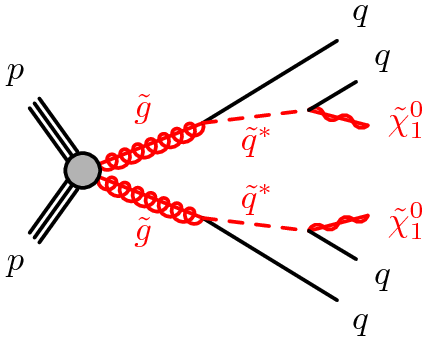
\includegraphics[width=0.5\textwidth]{figs/theory/T1qqqqLL}
\caption{Feynman diagram of long-lived gluino pair production, with each gluino 
decaying as $\gluino \rightarrow \mathrm{q}\bar{\mathrm{q}}\neutralino$ via a 
virtual squark \vsquark.}
\label{fig:T1qqqqLL}
\end{figure}

\begin{comment}
%The simulation of these models is described in Sec X.

%%%\subsection{Simplified models of supersymmetry}

%Feynman diagram of T1qqqqLL %(a) and dDM (need to make it myself?) (b)together.

%\subsection{Simplified models of dark matter}
%Buch.
%DMF, DMSimp?, dDM vector/axial

%Run 2 DM searches interpreted using simplified ``mono-X'' models with V/A/S/P 
%s-channel mediator pair decaying to Dirac fermion DM, with 4 parameters (two 
%masses and couplings).
%(Lagrangians probably not necessary)

%Extend these models to incorporate long-lived neutral particles. Kevin/me: 
%instead of mediator decaying to stable DM, it decays intermediate chi2 that is 
%long-lived and then chi2 decays to SM particles and stable DM. As chi2 
%%%lifetime 
%goes to infinity recover stable model.

%EFT description of chi2 decay. Lambda parameter can be swapped for lifetime 
%parameter.

%In this thesis consider model with vector mediator, couplings X and Y, and 
%various masses and lifetimes.


Define compressed and uncompressed? Mention ISR/FSR? (Adam/Baber)
\end{comment}

%\section{Status of experimental searches for dark matter and supersymmetry}
%\section{Status of searches for dark matter, supersymmetry and long-lived 
%particles}
\section{Status of searches for supersymmetry and long-lived particles}
\label{sec:theory-status}
%see rob lake louise
%many results out there but focus on those relevant to this thesis (displaced 
%jets, split susy/gluinos)
% current limits on vanilla/prompt susy, limit numbers on gluino, stop and lsp 
%(mt2, ra2b etc 36fb), therefore natural is now heavily constrained, however 
%still possibility that susy particles may be long lived as in split susy 
%scenario discussed previously
% therefore LL searches becoming more prominent now, example recent/strongest 
%limits on LL gluino/split susy, cms stopped, hscp, atlas displaced vertices, 
%mention/show limits of mass vs ctau, put rob ra1 plot in results to compare
%gluinos excluded almost 2 TeV, stops more than 1 TeV
Strong constraints have been placed by searches at the LHC on SUSY models with 
promptly decaying particles. Gluino and stop squark masses have been excluded 
up to approximately 2~TeV and 1~TeV, 
respectively~\cite{mt236,ra2b36,stop0L36,stop1L36,stop2L36}. 
This constrains the possibility of natural supersymmetry rather significantly.
%https://twiki.cern.ch/twiki/bin/view/CMSPublic/PhysicsResultsSUS

However, there is also the possibility that supersymmetric particles may be 
long-lived, as is the case of the gluino in the scenario of split supersymmetry 
discussed in Sec.~\ref{sec:theory-splitsusy}. Dedicated searches for exotic 
long-lived particles have therefore become more prominent at the LHC. Gluino 
lifetimes between 10~ps ($c\tau=1$~cm) and 100~ns ($\ctau=100$~m) have been 
excluded up to gluino masses in the range 1800-2400~GeV by a search in events 
with displaced vertices and missing energy in the ATLAS 
experiment~\cite{dispvert-atlas}. A search for jets from stopped gluinos in the 
CMS experiment has excluded the range of lifetimes between 100~ns 
($c\tau=100$~m) and 100~hours ($c\tau=100$~light-years) for gluino masses up to 
1385~GeV~\cite{stoppedgluino-cms}. Finally, the results of a CMS search for 
metastable gluinos (in the form of charged R-hadrons), that have lifetimes 
larger than the scale of the detector ($\tau \gtrsim 10$~ns, or $c\tau \gtrsim 
10$~m) exclude gluino masses up to 1850~GeV~\cite{hscp-cms}.
% 1 light year =~ 10^16 metres
% atlas: mlsp = 100 GeV, also has deltam=100 (mgluino limit drops to 1800)
%   https://atlas.web.cern.ch/Atlas/GROUPS/PHYSICS/PAPERS/SUSY-2016-08/
% stopped: deltam > 160 GeV
% hscp: lsp doesn't matter

The search presented in this thesis has been optimised for prompt decay 
signatures and does not employ specialised reconstruction techniques for 
long-lived particles. Nevertheless, it remains sensitive to events with LLPs 
and provides a complementary coverage to dedicated LLP searches, in particular 
for short lifetimes, as will be discussed in Chap.~\ref{chap:results}.
%as long as decays within tracker can still reconstruct with standard 
%algorithms, plus ISR)

%% my presentation
%Strong constraints have been set on “prompt” SUSY signatures
%The possibility that long-lived particles (LLPs) could be produced but remain 
%undetected is still open
%Most searches for LLPs so far have considered MET-less final states
%Want to see how sensitive a prompt MET search is, as well as complementarity 
%with displaced searches
%% my other presentation
%Easy to motivate LLPs – e.g. Split SUSY: decoupled squarks to high mass, 
%gluinos are long-lived, forming R-hadrons before decaying and giving rise to 
%final states with displaced jets and missing energy
%Present a novel interpretation of LL models with an inclusive search
%Broad and complementary coverage, in particular for sub-cm/sub-ns lifetimes 
%%%and compressed scenarios
%Also useful benchmark for dedicated searches

%very constrained hence look for LL signatures, we 
%think we’ve excluded X GeV gluinos but that’s not true if they’re LL.
%Mono-X but monojet strongest constraints.

%Current LL limits (CMS/ATLAS).
%Many possible types of striking signatures -- displaced leptons/photons/jets, 
%disappearing/kinked tracks, stopped particles, hscp, etc.
%Not many with MET, first LL interpretation of 
%prompt analysis (as long as decays within tracker can still reconstruct with 
%standard algorithms, plus ISR), briefly mention complementarity (sensitive to 
%whole range of lifetime, sub-cm and all mass splittings).

%see llp thesis and workshop
%https://indico.cern.ch/event/671803/
%LL searches: see paper (refs 36-46).